\documentclass[tikz,border=10pt]{standalone}
\usepackage{pgfplots}
\pgfplotsset{compat=1.16}

\begin{document}
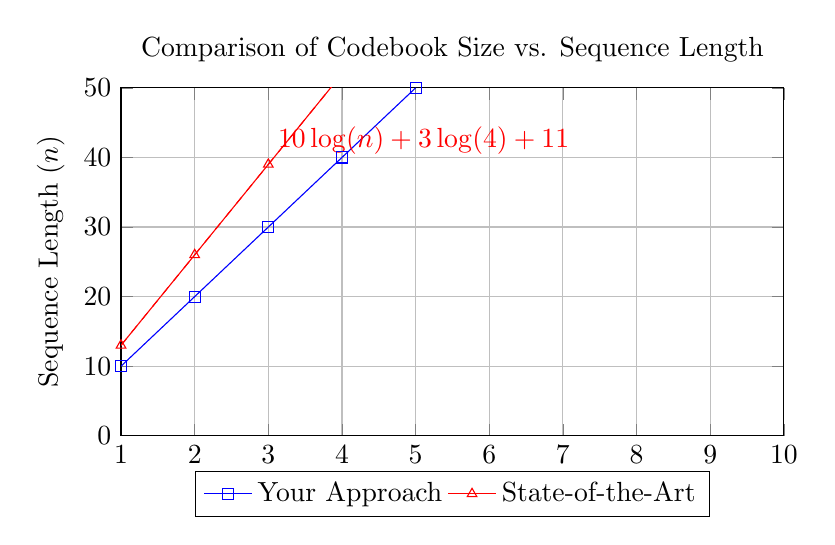
\begin{tikzpicture}
    \begin{axis}[
        title={Comparison of Codebook Size vs. Sequence Length},
        xlabel={Codebook Size},
        ylabel={Sequence Length ($n$)},
        ymin=0,
        ymax=50,
        xmin=1,
        xmax=10,
        xtick={1,2,3,4,5,6,7,8,9,10},
        ytick={0,10,20,30,40,50},
        grid=major,
        width=10cm,
        height=6cm,
        legend style={at={(0.5,-0.1)}, anchor=north,legend columns=-1}
    ]
        
        % Your approach data
        \addplot[blue, mark=square] coordinates {(1, 10) (2, 20) (3, 30) (4, 40) (5, 50)};
        \addlegendentry{Your Approach};
        
        % State-of-the-art data
        \addplot[red, mark=triangle] coordinates {(1, 13) (2, 26) (3, 39) (4, 52) (5, 65)};
        \addlegendentry{State-of-the-Art};
        
        % State-of-the-art formula
        \draw[dashed, red] (axis cs:1, 13) -- node[pos=0.5, above right] {$10\log(n) + 3\log(4) + 11$} (axis cs:5, 65);
        
    \end{axis}
\end{tikzpicture}
\end{document}